%\documentclass[12pt,a4paper,oneside,sumario=tradicional,brazil]{abntex2}
\documentclass[12pt,a4paper,oneside,sumario=tradicional,brazil]{abntex2}
\usepackage[utf8]{inputenc}
% set font arial
\usepackage{helvet}
\renewcommand{\rmdefault}{phv}
% set table colors
\usepackage[table]{xcolor}
%mesclando células vertical
\usepackage{multirow}
%colocando figuras
\usepackage{graphicx}
\usepackage{pdfpages}
\usepackage{float}
\usepackage{subfig}
% para plotagem de gráficos
\usepackage{pgfplots}   % pacote para uso do pgfplots
\pgfplotsset{width=1.0\linewidth,compat=1.11}
%\pgfplotsset{width=8cm,compat=1.11}
%\pgfplotsset{height=0.8\textheight,compat=1.11}
% pasta para imagens
\graphicspath{temp/imagens/}

% CONFIGURANDO CABEÇALHO
\makepagestyle{LRA}
\makeoddhead{LRA}{}{\scriptsize{\underline{[CABEÇALHO]} \\}}{\scriptsize{\underline{Página \thepage\ de \thelastpage}}}
%\makeevenhead{LRA}{}{\scriptsize{\underline{RA 0086-2014 Laudo de Avaliação Ambiental de Ruído – Cerâmica União Ituiutaba Ltda.  Outubro / 2014} \\}}{\scriptsize{\underline{Página \thepage\ de \thelastpage}}}
%\addtocounter{page}{1} % ADICIONANDO +1 PÁGINA PARA CONTAR A CAPA DO TRABALHO
% CONFIGURANDO CABEÇALHO - FIM

% CONFIGURANDO O ESTILO DO CABEÇALHO
\makechapterstyle{section}{
	\renewcommand{\printchaptername}{}
	\renewcommand{\chapternamenum}{}
	\renewcommand{\chaptitlefont}{\normalsize}
	\renewcommand{\chapnumfont}{\normalfont\normalsize\bfseries}
	\renewcommand{\printchapternum}{\chapnumfont \thechapter\space}
	\renewcommand{\afterchapternum}{}
	\renewcommand{\afterchapskip}{\onelineskip}
	\renewcommand{\beforechapskip}{0pt}
}
\renewcommand{\ABNTEXsectionfontsize}{\normalsize}

\chapterstyle{section}
% CONFIGURANDO O ESTILO DO CABEÇALHO - FIM


\begin{document}
%\textual
%\pagestyle{LRA}
%\aliaspagestyle{chapter}{LRA}

\

\vspace{5cm}
\begin{center}
	\textbf{\underline{{\HUGE CURRICULUM VITAE}}} \\
	\vspace{1cm}
	{\large Plínio Victor P. de Velloso Vianna}	
\end{center}

\newpage
\textual

Engenheiro Ambiental, nascido em 1989 (32 anos), formado ao final de 2013. Iniciou sua carreira de Técnico Ambiental na Empresa \textbf{QSE Consultoria e Assessoria LTDA}, sob a liderança de Euclides A. P. Lima e a Gerência de Pablo Kalil. \\
\indent
Realizou diversas atividades nesta empresa e em outras, dentre as quais destacam-se as \textit{Expertises} descritas neste documento. \\
\indent
Em função do encerramento das atividades da Empresa, ingressei como operador da Callink, no início do ano de 2021, inicialmente operador da Net/Claro, e posteriormente migrado à equipe do PagSeguro Atendimento Chat, quando tive a oportunidade de progredir para ser lotado no cargo de Assistente de Dados no setor de Inteligência da Informação que também realizei algumas atividades que se destacaram e posteriormente como Analista de Atendimento Jr do PagSeguro. \\
Atualmente estou em busca de novos desafios.

\begin{center}
	\textbf{{\Large Informações de contato}} \\
\end{center}
%\vspace{-1cm}
\begin{itemize}
	\item \textbf{Telefone:} (34) 9 8416-4207 \\
	\vspace{-1cm}
	\item \textbf{Telegram:} @pliniopvv \\
	\vspace{-1cm}
	\item \textbf{E-mail:} pliniopvv@gmail.com \\
	\vspace{-1cm}
	\item \textbf{LinkedId:} in/pliniopvv/ \\
	\vspace{-1cm}
	\item \textbf{GitHub:} /pliniopvv \\
\end{itemize}



\begin{center}
	\textbf{{\Large Formação Escolar}} \\
\end{center}
%\vspace{-1cm}
\begin{itemize}
	\item \textbf{Ensino Médio:} Escola Agrotécnica Federal de Rondônia. \\
	\vspace{-1cm}
	\item \textbf{Ensino Superior:} Iniciado na Universidade Federal de Rondônia e Concluído na Universidade de Uberaba, Campi Uberlândia. \\
\end{itemize}

\begin{center}
	\textbf{{\Large Habilidades}} \\
\end{center}
%\vspace{-1cm}
	\textbf{De escritório}: \\
	\vspace{-1cm}
\begin{itemize}
	\item Pacote Office Avançado - VisualBasicApplication. \\
	\vspace{-1cm}
	\item Libre Office Intermediário. \\
	\vspace{-1cm}
	\item Only Office Intermediário. \\
	\vspace{-1cm}
	\item Diagramação BPM. \\
\end{itemize}
	\textbf{De tecnologia}: \\
	\vspace{-1cm}
\begin{itemize}
	\item Java. \\
	\vspace{-1cm}
	\item NodeJS (ECMAScript/JavaScript) - Angular8, Express, TypeORM, NestJS. \\
	\vspace{-1cm}
	\item Python. \\
	\vspace{-1cm}
	\item SQL - MySQL, PostgreeSQL, JavaDB (atualmente MariaDB), Derby, H2. \\
	\vspace{-1cm}
	\item Arduino - ESP32, ESP8266, RaspberryPI. \\
\end{itemize}


%
%\begin{center}
%	\textbf{{\Large Expertise Profissional}} \\
%\end{center}
%\vspace{-1cm}

%Recém formado e contratado por uma empresa em formação, logo notou que o desafio exigiria mais do que sua formação. Na tentativa de aumentar a produtividade da equipe, desenvolveu-se diversos softwares administrativos, como oportunidade à empresa de melhorar sua produtividade, que foram eles: QseCapa, QseOS, QseClientesAdmin, GerOfícios dentre outros interrompidos. Também desenvolveu-se softwares para aumentar a produtividade das equipes em campo, como PvvRingelmann entre outros interrompidos. \\
%\pagebreak

\textbf{{\Large Contribuições extras:}} \\
\indent
A seguir listo alguns dos sistemas que desenvolvi como contribuições adicionais para solucionar problemas pontuais encontrados nos ambientes de trabalho pelos quais já passei.

\

\textbf{{\Large Softwares Administrativos}} \\
\indent
\textbf{{\large QseCapa}} \\
\indent
Notou-se a dificuldade de membros da equipe com softwares gráficos, portanto desenvolveu-se este aplicativo afim de simplificar a confecção das capas para os relatórios. \\
\indent
Aparência: \\
\begin{figure}[H]
	\centering
	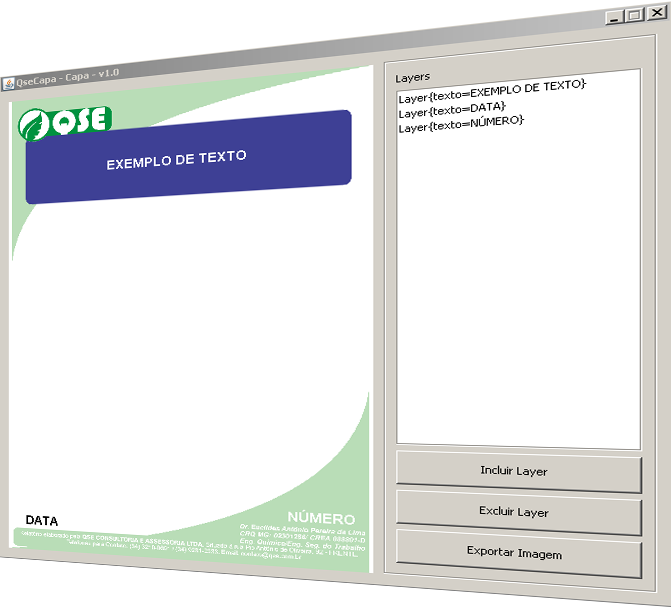
\includegraphics[width=0.4\linewidth]{imgs/QseCapa-aparencia-perspectiva.png}
	\caption{Tela principal do QseCapa}
\end{figure}
\indent
\textbf{{\large QseOS}} \\
\indent
A inexistência de um sistema para emissão de \textbf{Ordens de Serviço} criava dificuldades para a execução dos serviços em campo, por vezes também administrativos como a finalização dos relatórios. Para solucionar este problema criou-se o \textbf{QseOS}. Um software para a gestão de Ordens de Serviço. \\
\indent
Aparência: \\
	\begin{minipage}{\linewidth}
	\centering
	\begin{minipage}{0.45\linewidth}
		\begin{figure}[H]
			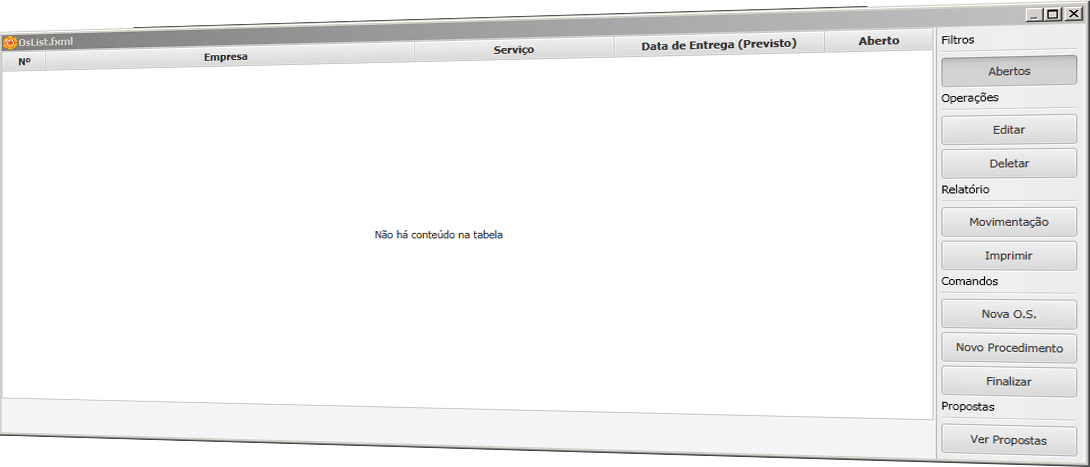
\includegraphics[width=8cm]{imgs/QseOS-principal.PNG}
			\caption{Tela Principal}
%			\ifnum #5 = 1
%			\label{foto_primeira}
%			\else
%			\fi
		\end{figure}
	\end{minipage}
	\hspace{0.05\linewidth}
	\begin{minipage}{0.45\linewidth}
		\begin{figure}[H]
			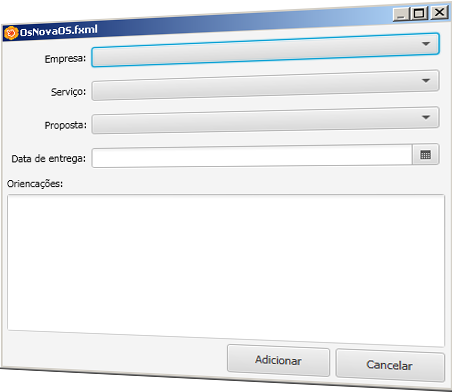
\includegraphics[width=8cm]{imgs/QseOS-criaros.PNG}
			\caption{Tela de criação}
%			\ifnum #5 = 2
%			\label{foto_ultima}
%			\else
%			\fi
		\end{figure}
	\end{minipage}
\end{minipage}

\textbf{QseClientesAdmin} \\
\indent
Os dados dos clientes ficavam constantemente desatualizados, portanto foi desenvolvido um sistema para centralizar as informações dos contatos em um banco de dados relacional (MySQL). \\
\indent
Aparência: \\
\begin{figure}[H]
	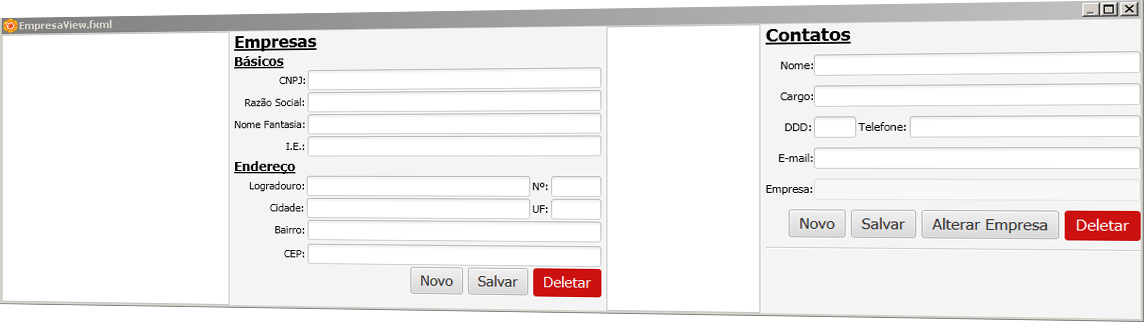
\includegraphics[width=1\linewidth]{imgs/QseClientesAdmin-telaprincipal.PNG}
	\caption{Tela principal do QseClientesAdmin}
\end{figure}

\textbf{GerOfícios} \\
\indent
O controle de ofícios era inexistente, portanto criou-se um software que ordenava e gerenciava os ofícios emitidos pela empresa. Deu-se o nome de 'GerOfícios'. \\
\indent
Aparência: \\
\begin{figure}[H]
	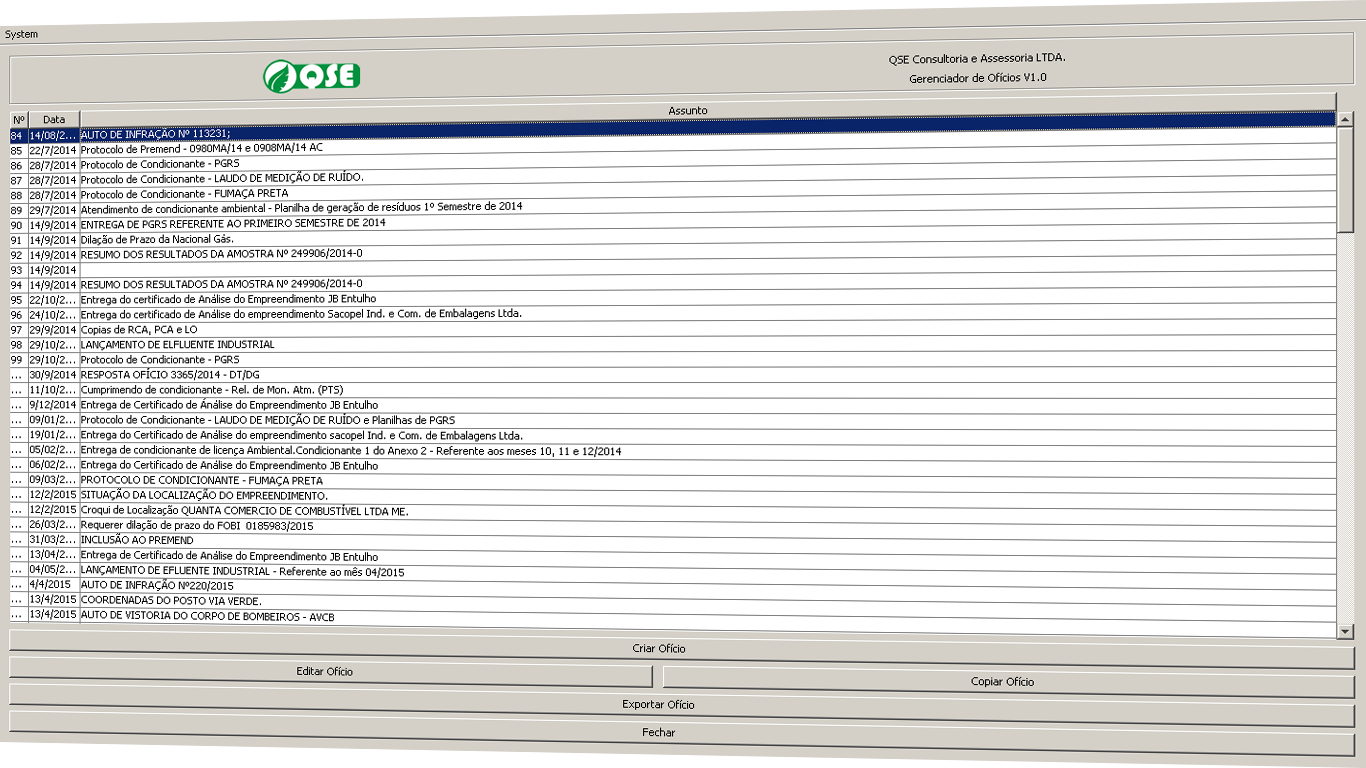
\includegraphics[width=1\linewidth]{imgs/GerOficios-principal.png}
	\caption{Tela principal do GerOfícios}
\end{figure}

%\begin{center}
	\textbf{{\large Expertise em campo}} \\
%\end{center}
	\indent
	Dentre as rotinas de campo estão a coleta e escrita de laudos de condicionantes ambientais, como: Ruído Ambiental, Material Particulado em Suspensão e Ringelmann. \\
	O laudo de Ruído Ambiental conforme determinam a NBR 10.151/2000, a Lei Estadual de 10.100/1990 e a Lei Municipal 10.700/2011. \\
	O laudo de Material Particulado em Suspensão conforme CONAMA 419/2018 que revogou a 03/1990. \\
	O laudo de Escala de Ringelmann conforme a Portaria Minter No 100, de 14 de Julho de 1980, Portaria do IBAMA No 85, de 17 de Outubro de 1996. \\
	
	\textbf{{\Large Softwares de campo}} \\
	\indent
	Desenvolveu-se um software para agilizar a escrita dos laudos de avaliação ambiental de ruído, porém a revisão do laudo desenvolvido pelo software ficou pendente, não chegando a ser utilizado. Como o software de Ruído não seguiu, não desenvolveu-se software para os laudos de Material Particulado. Porém o mesmo não ocorreu com o de Escala de Ringelmann. Desenvolveu-se dois softwares, um para Android e outro para Computador, que chamou-os, respectivamente de "PvvRingelmann" e "PvvBookmakerRingelmann" para a confecção destes laudos. \\
	\indent
	Aparência: \\
	\begin{minipage}{\linewidth}
		\centering
		\begin{minipage}{0.45\linewidth}
			\begin{figure}[H]
				\centering
				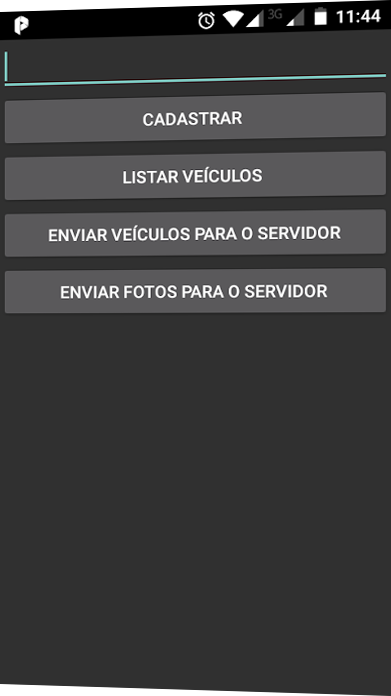
\includegraphics[width=4cm]{imgs/PvvRingelmann-principal.png}
				\caption{Tela Principal do software para Android}
				%			\ifnum #5 = 1
				%			\label{foto_primeira}
				%			\else
				%			\fi
			\end{figure}
		\end{minipage}
		\hspace{0.05\linewidth}
		\begin{minipage}{0.45\linewidth}
			\begin{figure}[H]
				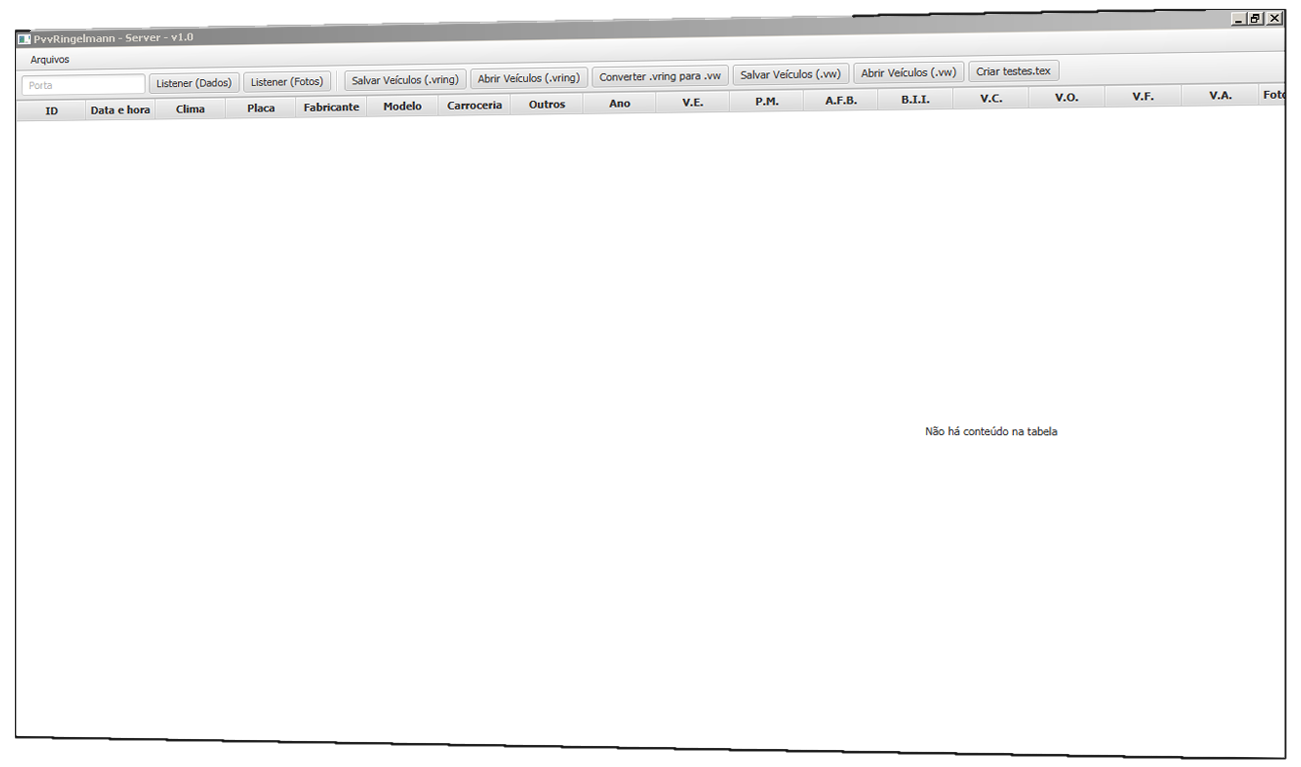
\includegraphics[width=8cm]{imgs/PvvBookmakerRingelmann-principal-border.png}
				\caption{Tela Principal do software para Computador}
				%			\ifnum #5 = 2
				%			\label{foto_ultima}
				%			\else
				%			\fi
			\end{figure}
		\end{minipage}
	\end{minipage} \\

%	\newpage
\

	
	\indent
	\textbf{{\large Operador de Atendimento - Pag Seguro}} \\
	\indent
	Inicialmente utilizando o Blip como ferramenta de atendimento, adicionei infirmações e indicadores complementares visuais que poderiam me auxiliar a cumprir com as regras de atendimento impostas ao operador, como última mensagem enviada e tempo total de atendimento do cliente que estava atendendo, recursos inexistentes na ferramenta. \\
	Migrada a ferramenta para o Genesys, desenvolvi botões-script, com scripts personalizados em que o operador teria a liberdade de realizar o cadastro de seus scripts na própria ferramenta locupleta campos que antes necessitariam serem digitados afim de agilizar respostas recorrentes. \\
	
	\indent
	
	\indent
	\textbf{{\large Assistente de Dados - MIS}} \\
	\indent
	Após ser operador de Atendimento na \textbf{Callink}, obtive a promoção para o cargo de \textbf{Assistente de Dados} cuja função era a execução de relatórios de inteligência para sobre as entregas da empresa para seus Clientes. Como rotina lidava muito com Macros em VBA e a limitação de ferramentas para desenvolvimento, utilizei o Powershell afim de poder realizar automações para agilizar a rotina que estava inserido, então desenvolvi um pequeno sistema demonstrado abaixo, baseado em símbolos e execução por comandos simples para manipulação dos relatórios baseados em excel sem que seja necessário a manipulação do excel diretamente. \\
	
	Aparência: \\
	\begin{minipage}{\linewidth}
		\centering
		\begin{minipage}{0.45\linewidth}
			\begin{figure}[H]
				\centering
				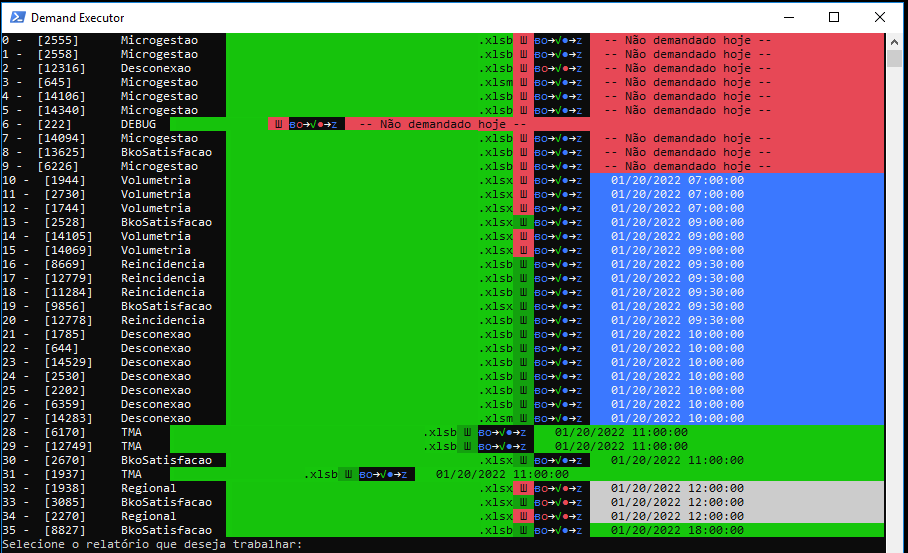
\includegraphics[width=8cm]{imgs/vbasis-mask.png}
				\caption{Tela Principal do sistema desenvolvido.}
				%			\ifnum #5 = 1
				%			\label{foto_primeira}
				%			\else
				%			\fi
			\end{figure}
		\end{minipage}
		\hspace{0.05\linewidth}
		\begin{minipage}{0.45\linewidth}
			\begin{figure}[H]
				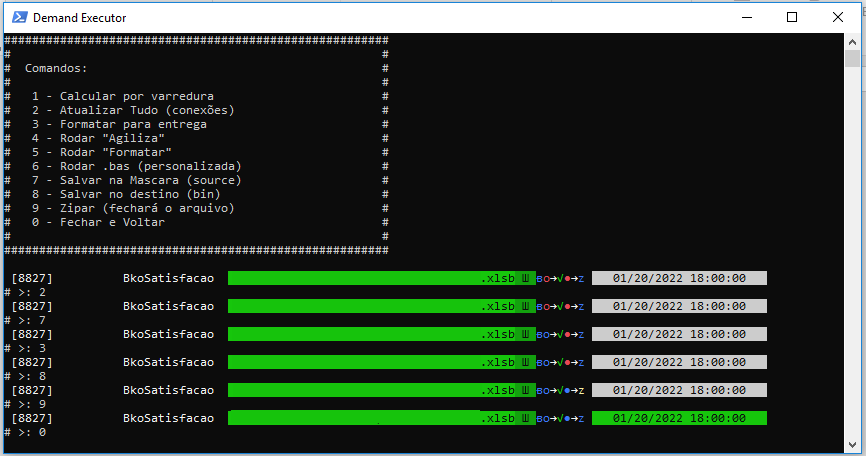
\includegraphics[width=8cm]{imgs/vbasisbuild-mask.png}
				\caption{Tela de confecção de um relatório.}
				%			\ifnum #5 = 2
				%			\label{foto_ultima}
				%			\else
				%			\fi
			\end{figure}
		\end{minipage}
	\end{minipage} \\

	\
	
	\indent
	\textbf{{\large Analista de Atendimento Jr - Pag Seguro.}} \\
	\indent
	
	Ao ter a oportunidade de trabalhar como Analista de Atendimento do PagSeguro, a rotina se baseava em analisar as dificuldades em solucionar os problemas dos Operadores de Atendimento com o material fornecido e locupletar as lacunas do material afim de concluir o atendimento iniciado. Esta rotina exigia a emissão de uma grande quantidade de disparos de e-mails com informações e solicitações para dar continuidade ao atendimento afim de poder cumprir com o tempo informado ao cliente na ponta. Para a realização desta tarefa foi desenvolvido o sistema abaixo em Python, afim de realizar a rotina de maneira mais ágil. \\
	
	Aparência: \\
	\begin{minipage}{\linewidth}
		\centering
		\begin{minipage}{0.45\linewidth}
			\begin{figure}[H]
				\centering
				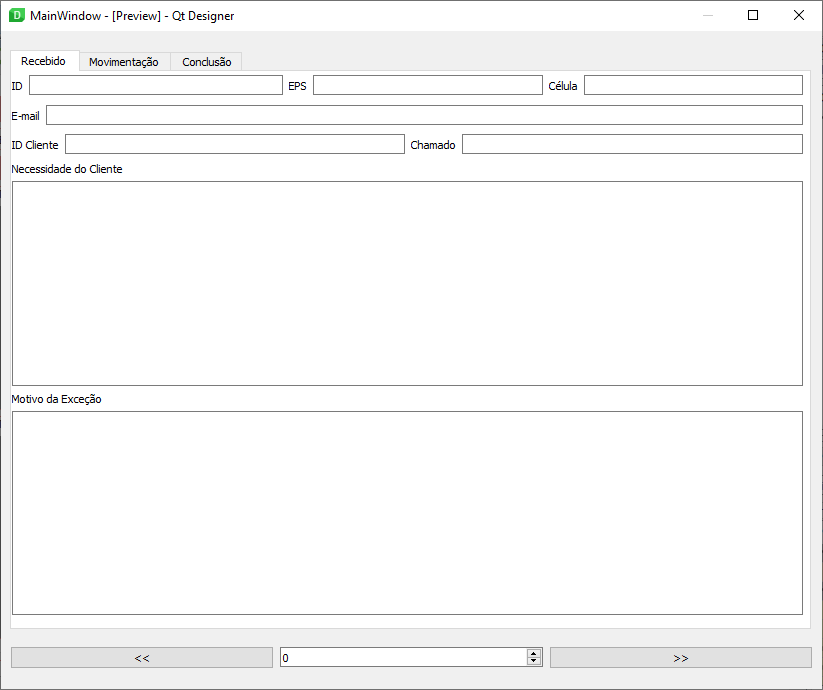
\includegraphics[width=8cm]{imgs/pagtrativa.png}
				\caption{Tela Principal do sistema desenvolvido.}
				%			\ifnum #5 = 1
				%			\label{foto_primeira}
				%			\else
				%			\fi
			\end{figure}
		\end{minipage}
		\hspace{0.05\linewidth}
		\begin{minipage}{0.45\linewidth}
			\begin{figure}[H]
				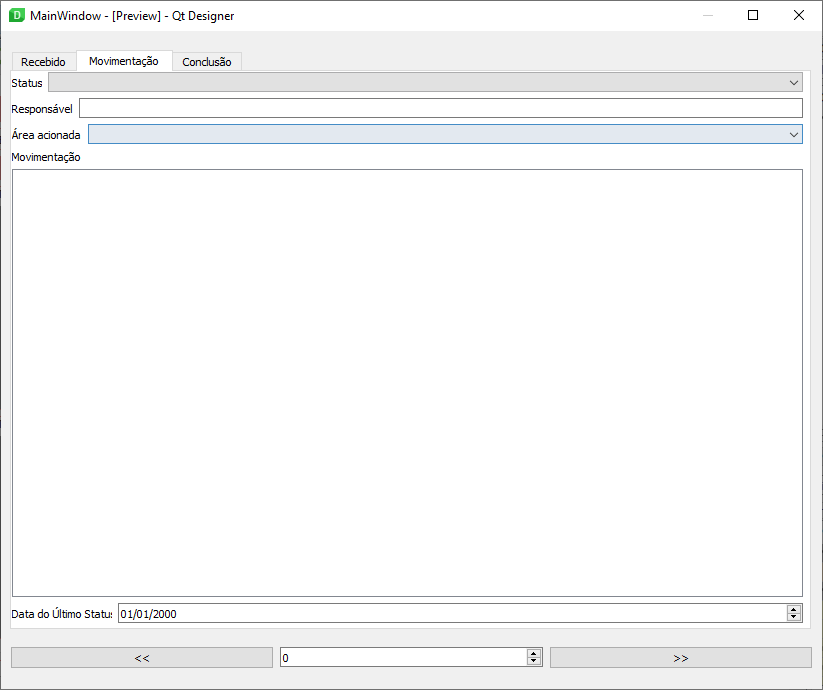
\includegraphics[width=8cm]{imgs/pagtrativatab2.png}
				\caption{Segunda tela de confecção de tratativa.}
				%			\ifnum #5 = 2
				%			\label{foto_ultima}
				%			\else
				%			\fi
			\end{figure}
		\end{minipage}
	\end{minipage} \\
	
	\
	
	\textbf{{\Large Colaborações em pesquisas científicas}} \\
	\indent
	\textbf{{\large PvvInmet}} \\
	\indent
	Aplicativo desenvolvido para realizar o download de dados das estações Automáticas do Inmet. O aplicativo ainda está em desenvolvimento. Com um ícone discreto próximo ao relógio, a aplicação realiza o download dos dados do último ano das estações selecionadas, para um banco de dados local. \\
	\indent
	Aparência: \\
	\begin{figure}[H]
		\centering
		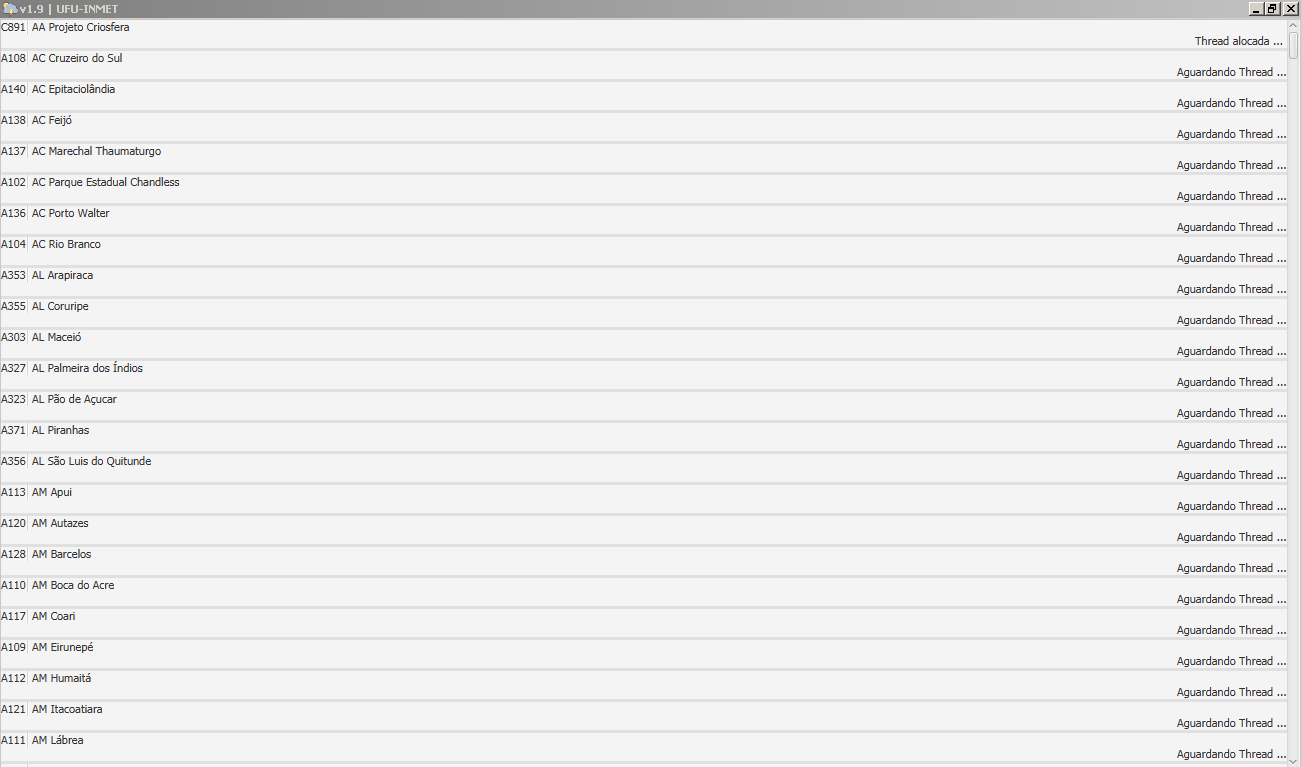
\includegraphics[width=0.9\linewidth]{imgs/pvvinmet-principal.PNG}
		\caption{Tela de Download das informações das estações}
	\end{figure}
	
	\
	
	\indent
	\textbf{{\large PvvUfu}} \\
	\indent
	Aplicativo desenvolvido para realizar a organização dos dados das estações Automáticas da Universidade Federal de Uberlândia. O aplicativo ainda está em desenvolvimento. Com um ícone discreto próximo ao relógio, a aplicação realiza o processamento dos logs das estações meteorológicas obtidas pelo operador. A intenção e aliar este software a Internet das Coisas e obter as informações diretamente do sensor. \\
	\indent
	Aparência: \\
		\begin{figure}[H]
			\centering
			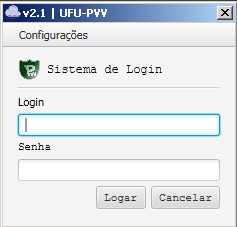
\includegraphics[width=0.25\linewidth]{imgs/pvvufu-tela-de-login.PNG}
			\caption{Tela de Login}
		\end{figure}
	
	\
	
	\indent
	\textbf{{\large Cidades inteligentes - IoT - Revolução Industral 4.0}} \\
	\indent
	Meu trabalho de conclusão de curso de titulo 'APLICAÇÃO DO ARDUINO PARA O MONITORAMENTO AMBIENTAL' foi aplicado no bairro 'Granja Marileusa'. Porém não teve continuidade em razão da ausência de apoio financeiro para o projeto. O trabalho consistia em realizar a transmissão de dados ambientais, inicialmente ruído, para um banco de dados por GPRS GSM 3G. \\
	\indent
%	Aparência: \\
%	\begin{figure}[H]
%		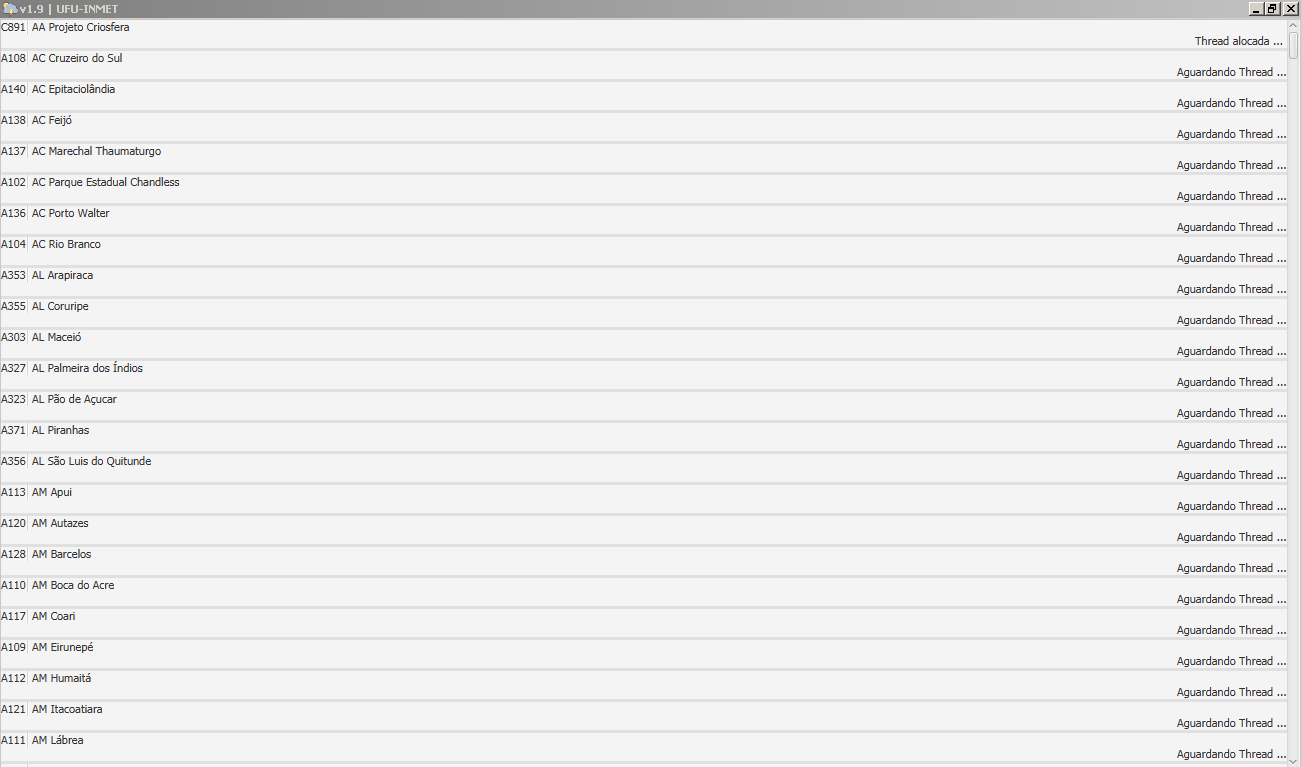
\includegraphics[width=1\linewidth]{imgs/pvvinmet-principal.PNG}
%		\caption{Tela de Download das informações das estações}
%	\end{figure}

	\
	
	
\end{document}